\documentclass[11pt]{beamer}
\let\Tiny=\tiny

\usefonttheme[onlymath]{serif}

\usepackage{multicol}
\usepackage{amssymb,amsmath,amsthm,stmaryrd}
\usepackage{indentfirst}
\usepackage{latexsym}
\usepackage[utf8]{inputenc}
\usepackage{fancybox}
\usepackage{tikz}
\usepackage{tikz-qtree}
\usepackage{multicol}
\usepackage{color}
\usepackage{eurosym}
\usepackage{listings}

\setbeamertemplate{navigation symbols}{}
\setbeamercovered{transparent}

\title[Language technologies and natural language processing]{A very short introduction to Language Technologies and Natural Language Processing}
\author{Jose F Quesada \& Jose Luis Pro}
\date{}

\mode<presentation>{\usetheme[]{Warsaw}}

\setbeamertemplate{footline}
    {
      \leavevmode
      \hbox{\begin{beamercolorbox}[wd=.5\paperwidth,ht=2.5ex,dp=1.125ex,leftskip=.3cm plus1fill,rightskip=.3cm]{author in head/foot}
        \usebeamerfont{author in head/foot}\insertshorttitle%
      \end{beamercolorbox}%
      \begin{beamercolorbox}[wd=.5\paperwidth,ht=2.5ex,dp=1.125ex,leftskip=.3cm,rightskip=.3cm plus1fil]{title in head/foot}
        \usebeamerfont{title in head/foot}
					\hfill\insertframenumber\,/\,\inserttotalframenumber
      \end{beamercolorbox}}
      \vskip0pt
    }

% TODO QUITAR AL FINAL
\hypersetup{pdfpagemode=UseNone}

\begin{document}

\begin{frame}
\titlepage
\end{frame}

\section{Preliminaries}
\subsection{Type of languages}

\begin{frame}
\setbeamercolor{block title}{use=structure,fg=white,bg=red!75!black}
\setbeamercolor{block body}{use=structure,fg=black,bg=red!10!white}
	\begin{block}{Language}
		\begin{center}
			Set of conventional spoken or written symbols used for commucation between entities.\par
			\pause
			So we can see a language as the linking between meaning (semantic side) and expression (syntantic side).
		\end{center}
	\end{block}
	\pause
	\vspace{15pt}
	Types of languages
	\begin{itemize}
		\item \textbf{Natural languages:} Used for the communication between human beings.
		\item \textbf{Formal languages:} Used by computers and in mathematical areas.
	\end{itemize}
\end{frame}

\begin{frame}
	\setbeamercolor{block title}{use=structure,fg=white,bg=red!75!black}
	\setbeamercolor{block body}{use=structure,fg=black,bg=red!10!white}
	\begin{block}{Differences between natural and formal languages:}
		\begin{enumerate}
			\pause
			\item Computers don't understand natural languages, (normal) humans don't understand computer languages.
			\item Formal languages shouldn't have ambiguities, but natural languages do have.
		\end{enumerate}
	\end{block} 
	\vspace{10pt}
	\pause 
	\textbf{Language Technologies} (LT's) are the set of technologies that aim to create software that has some kind of knowledge about natural languages. \par
	\vspace{10pt}
	\pause
	\textbf{Natural language processing} (NLP) is the scientific field concerned with the interactions between computers and human by means of natural languages.
\end{frame}

\subsection{Applications}

\begin{frame}
	\setbeamercolor{block title}{use=structure,fg=white,bg=blue!75!black}
	\setbeamercolor{block body}{use=structure,fg=black,bg=blue!10!white}
	\begin{block}{Applications of Language Technologies:}
		\begin{enumerate}
			\vspace{5pt}
			\item Machine Translation.
			\pause
			\item Question - Answering.
			\pause
			\item Automatic Text Classification.
			\pause
			\item Automatic Text Summarization.
			\pause
			\item Social Analytics.
			\pause
			\item Sentiment Analysis.
			\pause
			\item \textbf{Dialogue Systems.}
			\vspace{5pt}
		\end{enumerate}
	\end{block}
\end{frame}

\begin{frame}
	Dialogue Systems (written or spoken) are also known as:
	\begin{itemize}
		\item Conversational interfaces.
		\item Chatbots.
	\end{itemize}
	\vspace{20pt}
	\setbeamercolor{block title}{use=structure,fg=white,bg=blue!75!black}
	\setbeamercolor{block body}{use=structure,fg=black,bg=blue!10!white}
	\begin{block}{Applications of Dialogue Systems:}
		\begin{enumerate}
			\vspace{5pt}
			\pause
			\item Information providers.
			\pause
			\item Transactional agents.
			\pause
			\item Educational and learning tutoring.
			\vspace{5pt}
		\end{enumerate}
	\end{block}
\end{frame}
\subsection{Ambiguities}

\begin{frame}
	\setbeamercolor{block title}{use=structure,fg=white,bg=red!75!black}
	\setbeamercolor{block body}{use=structure,fg=black,bg=red!10!white}
	\begin{block}{Dialogue systems main issue}
		\begin{center}
		\vspace{10pt}
		The most difficult challenge in the design of conversational interfaces are related with the highly \\ambigous nature of spoken languages.
		\vspace{10pt}
		\end{center}
	\end{block}
	\setbeamercolor{block title}{use=structure,fg=white,bg=green!75!black}
	\setbeamercolor{block body}{use=structure,fg=black,bg=green!10!white}
	\pause	
	\begin{block}{Example}
		\begin{center}
		\vspace{10pt}
		\texttt{Peter come yesterday.}\par
		\texttt{Yesterday Peter come.}
		\vspace{10pt}
		\end{center}
	\end{block}
	\pause
	\begin{center}
		Two syntatic expressions $\Longleftrightarrow$ One semantic form
	\end{center}
\end{frame}

\begin{frame}
	\setbeamercolor{block title}{use=structure,fg=white,bg=green!75!black}
	\setbeamercolor{block body}{use=structure,fg=black,bg=green!10!white}
	\begin{block}{Example}
		\begin{center}
		\vspace{10pt}
		\texttt{Peter said John came yesterday.}
		\vspace{10pt}
		\end{center}
	\end{block}
	\vspace{10pt}
	\pause
	\begin{itemize}
		\item Was it yesterday when Peter said that?
		\item Was it yesterday when John came?
	\end{itemize}
	\vspace{10pt}
	\pause
	\begin{center}
		One syntatic expression $\Longleftrightarrow$ Two semantic forms
	\end{center}
\end{frame}

\begin{frame}
	Humans can deal with these ambiguities applying what is called ``psicolinguistic preferences'' and, of course, logic and common-sense reasoning:
	\vspace{10pt}
	\pause
	\setbeamercolor{block title}{use=structure,fg=white,bg=green!75!black}
	\setbeamercolor{block body}{use=structure,fg=black,bg=green!10!white}
	\begin{block}{Example}
		\begin{center}
		\vspace{10pt}
		\texttt{Peter said John will come yesterday.}
		\vspace{10pt}
		\end{center}
	\end{block}
	\vspace{10pt}
	\pause
	From the computer point of view this sentence is such ambigous like previous one but humans know that nobody \textsl{``will come yesterday''}.
\end{frame}

\subsection{Architecture}

\begin{frame}
\frametitle{Dialogue System architecture}
	\begin{center}
		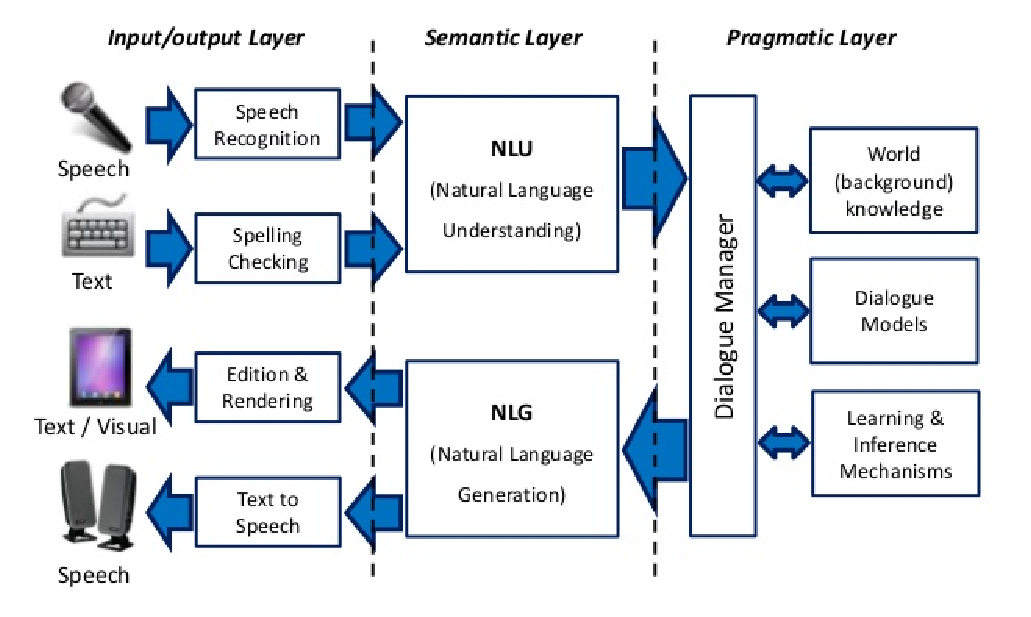
\includegraphics[width=1.00\textwidth]{ds.eps}
		\begin{tiny}
			Picture from Institute for Infocomm Research (Singapore)
		\end{tiny}
	\end{center}
\end{frame}

\section{Natural Language Understanding}
\subsection{Goal and meaning representation}

\begin{frame}
\frametitle{Natural Language Understanding (NLU)}
	\setbeamercolor{block title}{use=structure,fg=white,bg=red!75!black}
	\setbeamercolor{block body}{use=structure,fg=black,bg=red!10!white}
	\begin{block}{NLU main goal}
		\begin{center}
			\vspace{5pt}
			The goal of NLU stage is to transform an input string (let's say \textsl{user proference}) in an abstract representation of its meaning easier for computer programs to manipulate it, in order to execute some kind of reasoning.
			\vspace{5pt}
		\end{center}
	\end{block}
	\pause
	%\vspace{5pt}
	There is a wide variety of possible meaning representations.
	\begin{itemize}
		\item Topic maps.
		\item Concepts maps.
		\item Mind maps.
		\item Onthologies.
		\item \textbf{Feature structures.}
	\end{itemize}
\end{frame}

\begin{frame}
	\setbeamercolor{block title}{use=structure,fg=white,bg=green!75!black}
	\setbeamercolor{block body}{use=structure,fg=black,bg=green!10!white}
	\begin{block}{Example}
		\begin{center}
			\vspace{10pt}
				\texttt{John came yesterday} \small $\longrightarrow$ $\begin{bmatrix}
																				\textsc{Subject:}     & \texttt{John}\\ 
																				\textsc{Action:}      & \texttt{come}\\ 
																				\textsc{Tense:}     	& \texttt{past}\\ 
																				\textsc{Offsetdate:}  & \texttt{-1 day}\\ 
																			\end{bmatrix}$
			\vspace{10pt}
		\end{center}
	\end{block}
	\begin{block}{Example}
		\begin{center}
			\vspace{10pt}
				\texttt{John will talk in two days} \small $\longrightarrow$ $\begin{bmatrix}
																				\textsc{Subject:}     & \texttt{John}\\ 
																				\textsc{Action:}      & \texttt{talk}\\ 
																				\textsc{Tense:}     	& \texttt{future}\\ 
																				\textsc{Offsetdate:}  & \texttt{+2 day}\\ 
																			\end{bmatrix}$
			\vspace{10pt}
		\end{center}
	\end{block}
\end{frame}

\begin{frame}
	\setbeamercolor{block title}{use=structure,fg=white,bg=red!75!black}
	\setbeamercolor{block body}{use=structure,fg=black,bg=red!10!white}
	\begin{block}{Feature structures}
	\begin{itemize}
		\item A feature structure is a set of features.
		\item With no particular order between them.
		\item Every feature may have (but it's not required) an associated value.
		\item The value associated to every feature can be \textbf{atomic} or \textbf{complex}.
	\end{itemize}
	\end{block}
	\vspace{10pt}
	\pause
	\begin{center}
		\texttt{comes} \small $\longrightarrow$ 
				$\begin{bmatrix}
						\textsc{Action:}      & \texttt{come}\\ 
						\textsc{Tense:}     	& \texttt{present}\\ 
						\textsc{Agreement:}   & \begin{bmatrix}
																			\textsc{Number:} & \texttt{singular}\\ 
																			\textsc{Person:} & \texttt{3}\\ 
																		\end{bmatrix}
				\end{bmatrix}$
			\end{center}
\end{frame}

\subsection{NLU parts}

\begin{frame}
	\frametitle{NLU components}
	Trying to convert user proference to feature structures is not trivial. \par
	So we need to divide the process in some functional modules:
	\pause
	\vspace{10pt}
	\begin{itemize}
		\item Tokenization.
		\item Speller checker.
		\item Part Of Speech tagging (POS tagging).
		\item Parsing.
		\item Unifier.
	\end{itemize}
\end{frame}

\begin{frame}[fragile]
	\frametitle{Tokenization}
	\setbeamercolor{block title}{use=structure,fg=white,bg=red!75!black}
	\setbeamercolor{block body}{use=structure,fg=black,bg=red!10!white}
	\begin{block}{Goal}
		\begin{center}
			Convert a sequence of characters into a sequence of tokens.
		\end{center}
	\end{block}
	\pause
	We must take into account:
	\begin{itemize}
		\item Separators: \texttt{(\textvisiblespace -\char`_)}
		\item Punctuation marks: \texttt{(,.;:!?)}
		\item Special symbols: \texttt{(\$\euro\%º)}
		\item Numbers and its own separators: \texttt{(1234,.)}
		\item Alphanumeric codes: \texttt{(ES772024$\cdots$)}
	\end{itemize}
	\pause
	\setbeamercolor{block title}{use=structure,fg=white,bg=green!75!black}
	\setbeamercolor{block body}{use=structure,fg=black,bg=green!10!white}
	\begin{block}{Example}
	\begin{center}
		\begin{tabular}{ c c c c c c c c c c c c c c c c c }
			& tk1 & & tk2 & & tk3 & & tk4 & & tk5 & & tk6 \\
			$\cdot$ & The & $\cdot$ & dog & $\cdot$ & is & $\cdot$ & in & $\cdot$ & the & $\cdot$ & park & $\cdot$\\
			0 & & 1 & & 2 & & 3 & & 4 & & 5 & & 6
		\end{tabular}
	\end{center}
	\end{block}
\end{frame}

\begin{frame}
\frametitle{Speller checker (only in written dialogue systems)}
\begin{center}
	\Huge \texttt{London}
\end{center}
\begin{itemize}
	\item Insertion: \texttt{Loondon} 
	\item Deletion: \texttt{Lndon} 
	\item Substitution: \texttt{Lpndon} 
	\item Switching: \texttt{Lonodn} 
	\item Bad separators: \texttt{Lon don} 
\end{itemize}
\end{frame}

\begin{frame}
\frametitle{Part Of Speech tagging (POS tagging)}
	\setbeamercolor{block title}{use=structure,fg=white,bg=red!75!black}
	\setbeamercolor{block body}{use=structure,fg=black,bg=red!10!white}
	\begin{block}{Goal}
		\begin{center}
			To mark up lexical items with some lexical category depending on its definition and the context.
		\end{center}
	\end{block}
	\vspace{15pt}
	\pause
	In natural language we can have some common lexical categories:
	\begin{itemize}
		\item Determiners: \texttt{a, the} 
		\item Nouns: \texttt{London, dog} 
		\item Pronouns: \texttt{you, me} 
		\item Prepositions: \texttt{to, for} 
		\item Adjectives: \texttt{blue, long} 
	\end{itemize}
\end{frame}

\begin{frame}
\frametitle{POS tagging}
So in the lexicon definition we can classify lexical items into categories:\par
\begin{itemize}
	\item \texttt{("the", det)}
	\item \texttt{("dog", noun)}
	\item \texttt{("me", pronoun)}
	\item \texttt{("to", preposition)}
\end{itemize}
\vspace{5pt}
\pause
But in natural languages we can have several lexical categories corresponding to a single lexical item (especially in little inflectional ones, like in english): 
\begin{itemize}
	\item \texttt{("plans", noun)} $\longrightarrow$ plural of plan.
	\item \texttt{("plans", verb)} $\longrightarrow$ present of third person (singular) of verb to plan.
\end{itemize}
\end{frame}

\begin{frame}
\frametitle{POS tagging: Garden path problem}
	\setbeamercolor{block title}{use=structure,fg=white,bg=green!75!black}
	\setbeamercolor{block body}{use=structure,fg=black,bg=green!10!white}
	\begin{block}{Example}
		\begin{center}
		\begin{tabular}{ c c c c c c c c c c c c c c c c c }
			\underline{The} & \underline{\smash{government}} & \underline{\smash{plans}} & \underline{to} & \underline{raise} & \underline{taxes} & $\ldots$\\
			det & noun & \textbf{verb} & prep & verb & noun\\
		\end{tabular}
		\end{center}
	\end{block}
	\vspace{15pt}
	\pause
	\begin{block}{Example}
		\small
		\begin{center}
		\begin{tabular}{ c c c c c c c c c c c c c c c c c }
			\underline{The} & \underline{\smash{government}} & \underline{\smash{plans}} & \underline{to} & \underline{raise} & \underline{taxes} & \underline{were} & \underline{defeated}\\
			det & noun & \textbf{noun} & prep & verb & noun & verb & adj\\
		\end{tabular}
		\end{center}
	\end{block}
\end{frame}

\subsection{Grammars}

\begin{frame}
\end{frame}


%\begin{frame}
%\begin{center}
%\Tree [.S [.NP LaTeX ] [.VP [.V is ] [.NP fun ] ] ]
%\end{center}
%\end{frame}

\section{Dialogue Manager}

\begin{frame}
\end{frame}

\section{Natural Language Generation}

\begin{frame}
\end{frame}

\end{document}



